\section{Global Optimization}

Optimization is a field of applied mathematics that deals with finding the best
set of parameters to optimize an objective function. A problem with $N$
variables $\{n_0, \dots, n_{N-1}\}$ in range $n_i \in \{0, \dots, k-1\}$ will
have a search space with $k^N$ possible solutions. Each solution can be
evaluated by applying the objective function to it, to obtain the solutions
\emph{fitness}. The fitness is a measure of how good the solution is and it is
used to assist the selection of candidate solutions for evaluation.

The solution space can be thought of as a (N+1)-dimensional space that directly
relates to the number of variables in the solution, plus one axis for the
fitness value. E.g. when a problem contains a single variable, its solution
space might look like \autoref{fig:fitnesslandscape} where the X-axis is the
value of the single variable and the Y-axis is the fitness of this solution.
Problems with more variables will have more axis. The optimization algorithms
can be thought of as methods for exploring and finding the highest or lowest
point in of the fitness-axis.

As $k$ and $N$ grow large, it becomes infeasible to search through and
evaluate the vast amount of permutations and other techniques must be employed.
Finding an arbitrary local optimum is often straight forward using classical
\emph{local} optimization methods such as a simple hill climbing algorithm.
However, these methods cannot always be used to find a \emph{global} optimum. A wide
range of algorithms to search through a subset of the solution space exists,
each with different approaches and properties. Many of these are described in
detail in \cite{russellnorvig}.

\begin{figure}[bth]
    \centering
    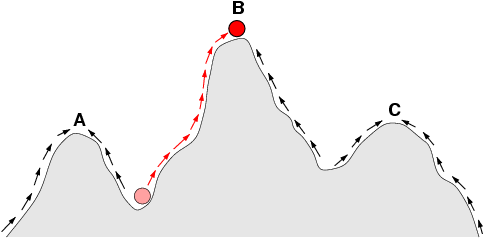
\includegraphics[width=0.8\textwidth]{figs/Fitness-landscape-cartoon.png}
    \caption{A one-dimensional fitness landscape. The arrows indicate the
        preferred flow of a population on the landscape, and the points A and C
        are local optima. The red ball indicates a population that moves from a
        very low fitness value to the top of a peak. Borrowed from \cite{wikifitnesslandscape}.}
    \label{fig:fitnesslandscape}
\end{figure}

On a high level, optimization algorithms can be divided into deterministic and
non-deterministic approaches. The deterministic approaches can be thought of as
a single path in solution space that starts at a defined but most likely
suboptimal solution and ends at the best solution. The non-deterministic
approaches usually selects one or more paths at random such that each run might
yields a different outcome. Deterministic algorithms will always find the same
solution, but if the search space is large this might be extremely time
consuming. With the case of non-deterministic algorithms, they tend to have
an explorative behaviour \cite{poli2008field}; each computation of next state
includes some form of randomness. E.g. simulated annealing will do the same as
the hill climbing algorithm, but will have some chance of moving downhill, thus
it will be less prone to be stuck in a local optimum. We will now provide a brief
overview of algorithms considered for use in this thesis.


\begin{description}
    \item[Regression] is described as a study of dependence between properties
        \cite{weisberg2005applied}. When data set contains values from at
        least two properties, regression can be used to find one value as a
        function of the other. The simplest form of regression is the linear
        regression. A linear regression will try to find the linear function,
        $y=a_1x_1+a_2x_2+...+a_nx_n+b$, that minimizes the least square error.
        Common for implementation of linear regression solvers is to formulate
        the problem as a system of linear equations \cite{lay2011linear}, which
        can be solved by Gaussian elimination. More advanced forms for
        regressions can be used when the problem cannot be well mapped with a
        linear function, such as the Gauss-Newton algorithm
        \cite{myers1990classical}.

    \item[Simulated Annealing] is a technique that belongs to the field of
        stochastic optimization and metaheuristics, inspired by the process of
        annealing in metallurgy \cite{van1987simulated}. Initially, it starts in
        a random state $s$ and for each iteration it probabilistically decides
        between moving the system to a neighboring state $s'$ or staying in
        state $s$. To avoid ending up in a local optimum, the probability starts
        high, but decreases over time. Hence, simulated annealing can quickly
        consider the most important parts of the state if configured adequately.

    \item[Evolutionary Algorithms] is a term that refers to computational
        methods inspired by the process and mechanisms of biological evolution
        \cite{fogel1997evolutionary}.  They differ from conventional algorithms
        by selecting the best-fit individuals in a population for reproduction
        and applying crossover and mutation to produce offspring. Only the best
        fit individuals go on to the next generation \cite{introtoga}.

\end{description}

Global optimization problems are a well studied research area and there is a
wealth of different ways to solve them. It can be difficult to know in advance
which methods will provide the most fruitful results. Also, multiple approaches
can be combined in efforts to extract the best properties from several worlds,
or to get the speed of convergence up.

In this thesis, we have chosen to use an evolutionary approach called $1 +
\lambda$, with $\lambda = 4$. It includes the following steps:

\begin{enumerate}
    \item Generate $\lambda$ random individuals.
    \item Evaluate population.
    \item Select the best individual.
    \item Mutate $\lambda$ new individuals from the most-fit induvidual.
    \item Repeat step 2 through 4 for each generation.
\end{enumerate}

